% Options for packages loaded elsewhere
\PassOptionsToPackage{unicode}{hyperref}
\PassOptionsToPackage{hyphens}{url}
%
\documentclass[
  doc,floatsintext]{apa6}
\usepackage{amsmath,amssymb}
\usepackage{iftex}
\ifPDFTeX
  \usepackage[T1]{fontenc}
  \usepackage[utf8]{inputenc}
  \usepackage{textcomp} % provide euro and other symbols
\else % if luatex or xetex
  \usepackage{unicode-math} % this also loads fontspec
  \defaultfontfeatures{Scale=MatchLowercase}
  \defaultfontfeatures[\rmfamily]{Ligatures=TeX,Scale=1}
\fi
\usepackage{lmodern}
\ifPDFTeX\else
  % xetex/luatex font selection
\fi
% Use upquote if available, for straight quotes in verbatim environments
\IfFileExists{upquote.sty}{\usepackage{upquote}}{}
\IfFileExists{microtype.sty}{% use microtype if available
  \usepackage[]{microtype}
  \UseMicrotypeSet[protrusion]{basicmath} % disable protrusion for tt fonts
}{}
\makeatletter
\@ifundefined{KOMAClassName}{% if non-KOMA class
  \IfFileExists{parskip.sty}{%
    \usepackage{parskip}
  }{% else
    \setlength{\parindent}{0pt}
    \setlength{\parskip}{6pt plus 2pt minus 1pt}}
}{% if KOMA class
  \KOMAoptions{parskip=half}}
\makeatother
\usepackage{xcolor}
\usepackage{graphicx}
\makeatletter
\def\maxwidth{\ifdim\Gin@nat@width>\linewidth\linewidth\else\Gin@nat@width\fi}
\def\maxheight{\ifdim\Gin@nat@height>\textheight\textheight\else\Gin@nat@height\fi}
\makeatother
% Scale images if necessary, so that they will not overflow the page
% margins by default, and it is still possible to overwrite the defaults
% using explicit options in \includegraphics[width, height, ...]{}
\setkeys{Gin}{width=\maxwidth,height=\maxheight,keepaspectratio}
% Set default figure placement to htbp
\makeatletter
\def\fps@figure{htbp}
\makeatother
\setlength{\emergencystretch}{3em} % prevent overfull lines
\providecommand{\tightlist}{%
  \setlength{\itemsep}{0pt}\setlength{\parskip}{0pt}}
\setcounter{secnumdepth}{-\maxdimen} % remove section numbering
% Make \paragraph and \subparagraph free-standing
\ifx\paragraph\undefined\else
  \let\oldparagraph\paragraph
  \renewcommand{\paragraph}[1]{\oldparagraph{#1}\mbox{}}
\fi
\ifx\subparagraph\undefined\else
  \let\oldsubparagraph\subparagraph
  \renewcommand{\subparagraph}[1]{\oldsubparagraph{#1}\mbox{}}
\fi
\newlength{\cslhangindent}
\setlength{\cslhangindent}{1.5em}
\newlength{\csllabelwidth}
\setlength{\csllabelwidth}{3em}
\newlength{\cslentryspacingunit} % times entry-spacing
\setlength{\cslentryspacingunit}{\parskip}
\newenvironment{CSLReferences}[2] % #1 hanging-ident, #2 entry spacing
 {% don't indent paragraphs
  \setlength{\parindent}{0pt}
  % turn on hanging indent if param 1 is 1
  \ifodd #1
  \let\oldpar\par
  \def\par{\hangindent=\cslhangindent\oldpar}
  \fi
  % set entry spacing
  \setlength{\parskip}{#2\cslentryspacingunit}
 }%
 {}
\usepackage{calc}
\newcommand{\CSLBlock}[1]{#1\hfill\break}
\newcommand{\CSLLeftMargin}[1]{\parbox[t]{\csllabelwidth}{#1}}
\newcommand{\CSLRightInline}[1]{\parbox[t]{\linewidth - \csllabelwidth}{#1}\break}
\newcommand{\CSLIndent}[1]{\hspace{\cslhangindent}#1}
\ifLuaTeX
\usepackage[bidi=basic]{babel}
\else
\usepackage[bidi=default]{babel}
\fi
\babelprovide[main,import]{english}
% get rid of language-specific shorthands (see #6817):
\let\LanguageShortHands\languageshorthands
\def\languageshorthands#1{}
% Manuscript styling
\usepackage{upgreek}
\captionsetup{font=singlespacing,justification=justified}

% Table formatting
\usepackage{longtable}
\usepackage{lscape}
% \usepackage[counterclockwise]{rotating}   % Landscape page setup for large tables
\usepackage{multirow}		% Table styling
\usepackage{tabularx}		% Control Column width
\usepackage[flushleft]{threeparttable}	% Allows for three part tables with a specified notes section
\usepackage{threeparttablex}            % Lets threeparttable work with longtable

% Create new environments so endfloat can handle them
% \newenvironment{ltable}
%   {\begin{landscape}\centering\begin{threeparttable}}
%   {\end{threeparttable}\end{landscape}}
\newenvironment{lltable}{\begin{landscape}\centering\begin{ThreePartTable}}{\end{ThreePartTable}\end{landscape}}

% Enables adjusting longtable caption width to table width
% Solution found at http://golatex.de/longtable-mit-caption-so-breit-wie-die-tabelle-t15767.html
\makeatletter
\newcommand\LastLTentrywidth{1em}
\newlength\longtablewidth
\setlength{\longtablewidth}{1in}
\newcommand{\getlongtablewidth}{\begingroup \ifcsname LT@\roman{LT@tables}\endcsname \global\longtablewidth=0pt \renewcommand{\LT@entry}[2]{\global\advance\longtablewidth by ##2\relax\gdef\LastLTentrywidth{##2}}\@nameuse{LT@\roman{LT@tables}} \fi \endgroup}

% \setlength{\parindent}{0.5in}
% \setlength{\parskip}{0pt plus 0pt minus 0pt}

% Overwrite redefinition of paragraph and subparagraph by the default LaTeX template
% See https://github.com/crsh/papaja/issues/292
\makeatletter
\renewcommand{\paragraph}{\@startsection{paragraph}{4}{\parindent}%
  {0\baselineskip \@plus 0.2ex \@minus 0.2ex}%
  {-1em}%
  {\normalfont\normalsize\bfseries\itshape\typesectitle}}

\renewcommand{\subparagraph}[1]{\@startsection{subparagraph}{5}{1em}%
  {0\baselineskip \@plus 0.2ex \@minus 0.2ex}%
  {-\z@\relax}%
  {\normalfont\normalsize\itshape\hspace{\parindent}{#1}\textit{\addperi}}{\relax}}
\makeatother

\makeatletter
\usepackage{etoolbox}
\patchcmd{\maketitle}
  {\section{\normalfont\normalsize\abstractname}}
  {\section*{\normalfont\normalsize\abstractname}}
  {}{\typeout{Failed to patch abstract.}}
\patchcmd{\maketitle}
  {\section{\protect\normalfont{\@title}}}
  {\section*{\protect\normalfont{\@title}}}
  {}{\typeout{Failed to patch title.}}
\makeatother

\usepackage{xpatch}
\makeatletter
\xapptocmd\appendix
  {\xapptocmd\section
    {\addcontentsline{toc}{section}{\appendixname\ifoneappendix\else~\theappendix\fi\\: #1}}
    {}{\InnerPatchFailed}%
  }
{}{\PatchFailed}
\usepackage{csquotes}
\usepackage{placeins} 

\ifLuaTeX
  \usepackage{selnolig}  % disable illegal ligatures
\fi
\IfFileExists{bookmark.sty}{\usepackage{bookmark}}{\usepackage{hyperref}}
\IfFileExists{xurl.sty}{\usepackage{xurl}}{} % add URL line breaks if available
\urlstyle{same}
\hypersetup{
  pdftitle={Who mistrust basic science?},
  pdfauthor={Jan Pfänder1, Lou Kerzreho1, \& Hugo Mercier1},
  pdflang={en-EN},
  hidelinks,
  pdfcreator={LaTeX via pandoc}}

\title{Who mistrust basic science?}
\author{Jan Pfänder\textsuperscript{1}, Lou Kerzreho\textsuperscript{1}, \& Hugo Mercier\textsuperscript{1}}
\date{}


\shorttitle{Who mistrust basic science?}

\authornote{

HM received funding from the ANR (SCALUP, ANR-21-CE28-0016-01), and from the John Tempelton Foundation (``An Evolutionary and Cultural Perspective on Intellectual Humility via Intellectual Curiosity and Epistemic Deference''). The ANR also supported this project through FrontCog (ANR-17-EURE-0017), and PSL (ANR-10-IDEX-0001-02).

The authors made the following contributions. Jan Pfänder: ; Lou Kerzreho: ; Hugo Mercier: .

Correspondence concerning this article should be addressed to Hugo Mercier, . E-mail: \href{mailto:hugo.mercier@gmail.com}{\nolinkurl{hugo.mercier@gmail.com}}

}

\affiliation{\vspace{0.5cm}\textsuperscript{1} Institut Jean Nicod, Département d'études cognitives, ENS, EHESS, PSL University, CNRS, France}

\abstract{%
XX
}



\begin{document}
\maketitle

\hypertarget{introduction}{%
\section{Introduction}\label{introduction}}

There is increasingly more talk of defiance towards science and towards experts more generally (for science, see the intro to the stability paper, see also Paresman et al on populism?). In every population, many people only trust science `some of the time', and a sizable minority doesn't trust it.

This appears difficult to reconcile with the fact that, in many countries, most people receive at least a basic science education, that science education (along with education more generally) is increasing, and that science education seems to be the main driver of trust in science.

But how deep is distrust of science? Do people reject science wholesale, or is it more driven by attitudes towards specific contents, maybe in particular those seen as being politicized, or as going against deeply held beliefs, or behaviors they want to engage in? {[}previous work suggests that issue-specific claims provoke more negative attitudes{]}

Here, we look at whether people, across different levels of trust in science (and of other relevant attitudes? Conspi? Populists? Apparently on Prolific we can specifically target antivax people for instance, which could be quite useful), accept basic scientific facts.

{[}We can draw some inspiration from the ``Westwood et al 2021 Current research overstates American support for political violence'' paper: we want to put in perspective the current rise (? discourse around?) in mistrust towards science{]}

\hypertarget{levels-of-trust-in-science}{%
\subsection{Levels of trust in science}\label{levels-of-trust-in-science}}

\hypertarget{why-do-people-distrust-science}{%
\subsection{Why do people distrust science?}\label{why-do-people-distrust-science}}

{[}here? We know from the many studies on the gateway belief model that people don't always accept the scientific consensus (indeed, the effect sizes are usually not massive){]}

\hypertarget{how-much-science-do-people-know}{%
\subsection{How much science do people know?}\label{how-much-science-do-people-know}}

This is a crucial point: if there are questions with specific scientific answers that just about everyone already knows, then in a sense our point is already proven\ldots{} so the first thing to do would be to look at data on knowledge of science, and see what the highest rates of correct answer is, to see how much room for improvement there is.

``The dominant approach to conceptualizing and measuring science literacy in population surveys has arisen out of work by Jon D. Miller and Kenneth Prewitt in the United States (see Miller, 1983, 1998, 2004) alongside collabora- tors in Great Britain (see Durant et al., 1989). Underlying these efforts appears to have been widespread concern among policy makers and the scientific com- munity that nonscientists were becoming skeptical about the benefits of sci- ence and that such skepticism might result in cuts to science funding that would harm the scientific progress that many argue underpins both American and European economic development (Bauer et al., 2007). The results of the U.S. portion of this work have formed the core of a chapter of a biennial report called Science and Engineering Indicators (hereafter, Indicators) that the National Science Board provides to Congress and the Executive Branch. Scholars have also used the raw data collected for Indicators (which is made publicly available) for peer-reviewed research (e.g., Gauchat, 2012; Losh, 2010), and other countries have used many of the Indicators' questions for their own national surveys (e.g., Bauer et al., 2012a; National Science Board, 2016).''

\hypertarget{first-series-of-experiments}{%
\section{First series of experiments}\label{first-series-of-experiments}}

The goal is to see how many people really don't accept basic science (in practice, get as close to ceiling in acceptance as we can, first with a generic sample, then see if that still works with an anti-vax sample).

\hypertarget{experiment-1}{%
\section{Experiment 1}\label{experiment-1}}

The main goal of experiment one was to test whether people would accept the scientific consensus on basic knowledge questions. Additionally, we wanted to know if both science knowledge and acceptance of the scientific consensus are associated with trust in science and conspiracy thinking. We had the following research questions:

\begin{itemize}
\item
  \textbf{RQ1: What is the average science knowledge score (1)?}
\item
  \textbf{RQ2: What is the average acceptance of the scientific consensus (2)?}
\item
  \textbf{RQ3: What is the relationship between trust in science and, respectively, (1) and (2)?}
\item
  \textbf{RQ4: What is the relationship between conspiracy thinking and, respectively, (1) and (2)?}
\end{itemize}

\hypertarget{methods}{%
\subsection{Methods}\label{methods}}

\hypertarget{participants}{%
\subsubsection{Participants}\label{participants}}

We recruited 200 participants from the US via prolific. 6 participants failed our attention check, resulting in a final sample of 194 participants (98 female, 96 male; \(age_\text{mean}\): 41.71, \(age_\text{sd}\): 13.07, \(age_\text{median}\): 39). Since we did not have any prior assumptions on effect sizes, we did not do a power analysis.

\hypertarget{procedure}{%
\subsubsection{Procedure}\label{procedure}}

After providing their consent to participate in the study, participants were given an attention check ``While watching the television, have you ever had a fatal heart attack?'' {[}1-6; 1 = Never, 6 = Often{]}. All participants who did not answer ``1 = Never'' were excluded. Participants then read the following instructions:``We will ask you 11 questions about science. After each question, we will provide you with the scientifically consensual answer and ask whether you accept it.'' Next, participants answered a set of 10 basic science questions, which were randomly selected from a pool of 11 questions, in random order. After each question, participants were presented with an answer reflecting the scientific consensus. Participants were asked to choose whether they accept the answer or not, before proceeding to the next question. Figure \ref{fig:stimulus-example} displays the survey for an example science question. Finally, participants answered questions on conspiracy thinking and trust in science.



\begin{figure}

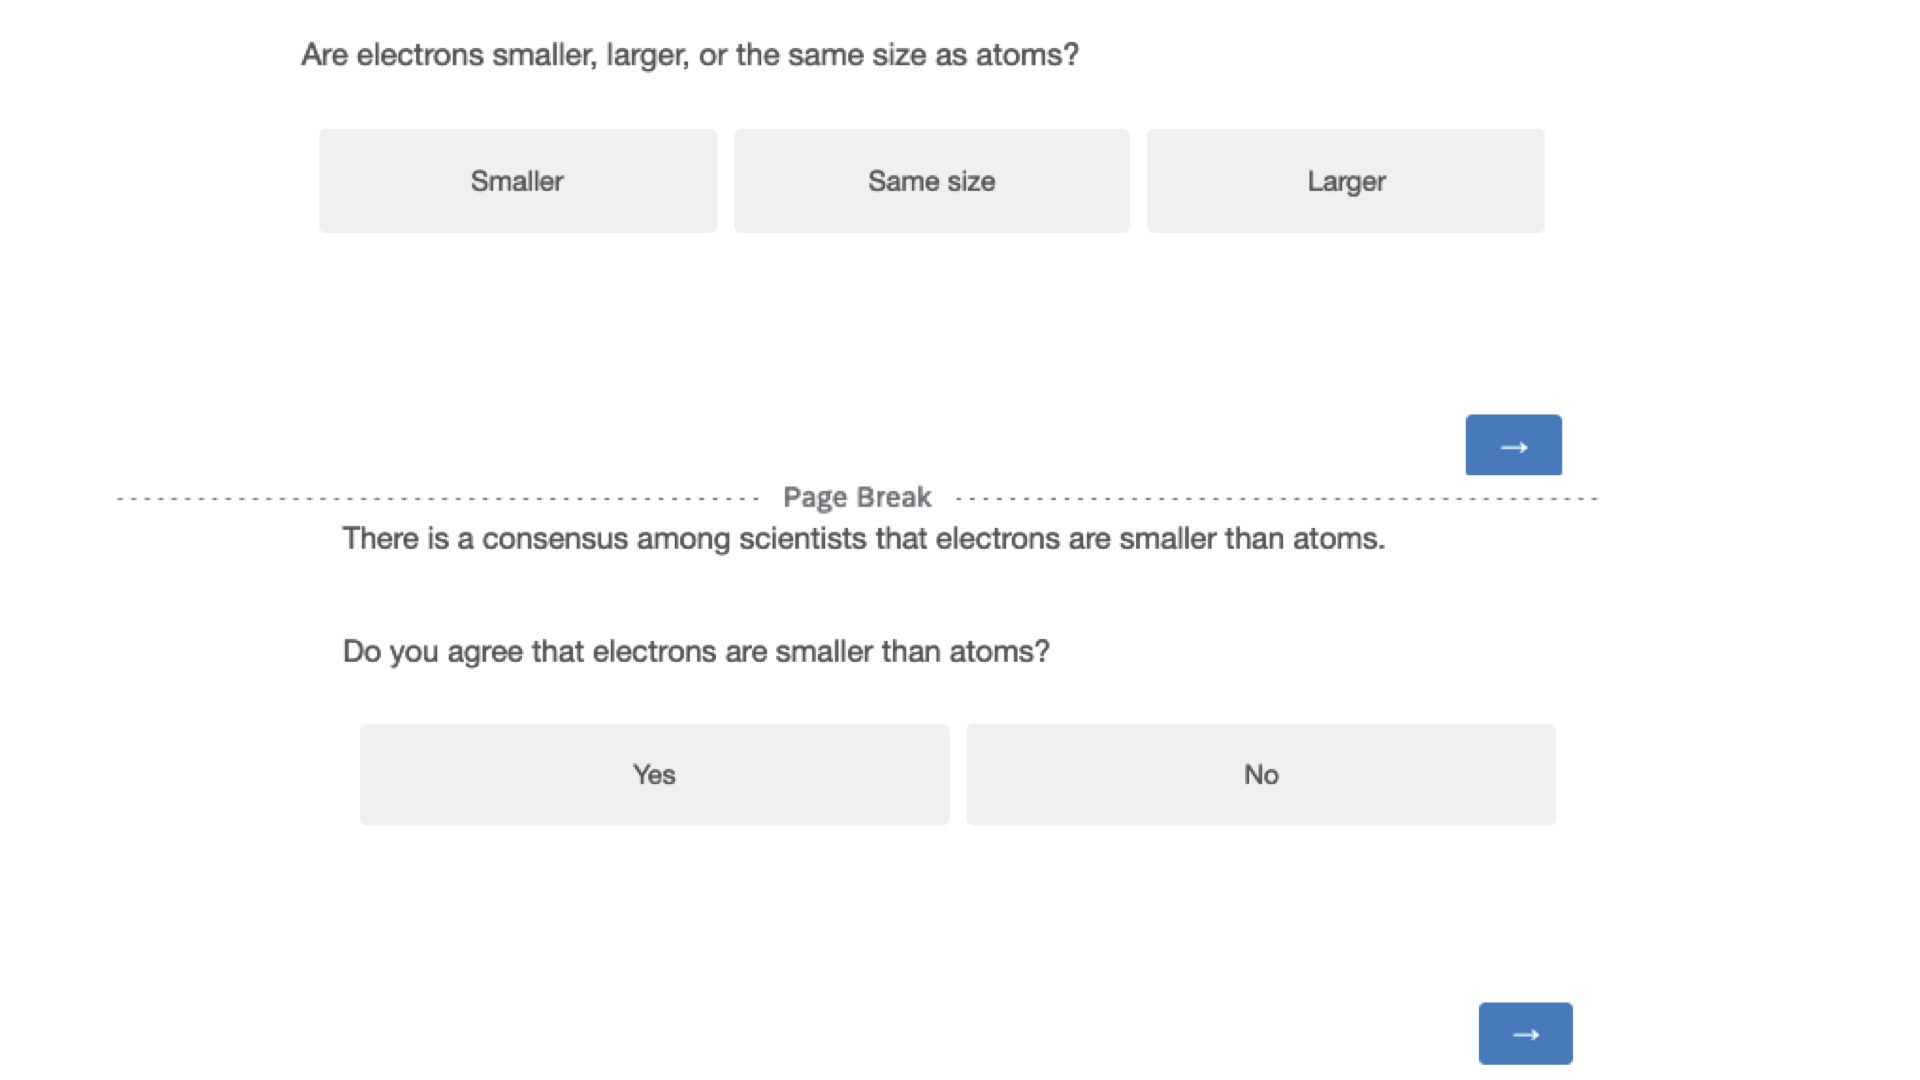
\includegraphics[width=1\linewidth]{./figures/study1_question_example} \hfill{}

\caption{Example of a science question, the scientific consensus and the corresponding acceptance question.}\label{fig:stimulus-example}
\end{figure}

\hypertarget{materials}{%
\subsubsection{Materials}\label{materials}}

\hypertarget{science-knowledge-and-acceptance}{%
\paragraph{Science knowledge and acceptance}\label{science-knowledge-and-acceptance}}

Table \ref{tab:knowledge} shows all questions, their scientifically consensual answer, and their source. All but two questions were selected from existing science knowledge questionnaires. We tried to select non-political questions.

\begin{longtable}[t]{>{\raggedleft\arraybackslash}p{1em}>{\raggedright\arraybackslash}p{10em}>{\raggedright\arraybackslash}p{10em}>{\raggedright\arraybackslash}p{15em}}
\caption{\label{tab:knowledge}Science knowledge items}\\
\toprule
id & Question & Scientific consensus & Reference(s)\\
\midrule
1 & Do antibiotics kill viruses as well as bacteria? & There is a consensus among scientists that antibiotics kill bacteria, but not viruses. & (Sturgis \& Allum, 2004), (Miller, 2004), (Miller, 1998) (Tourangeau et al., 2016), (Evans \& Durant, 1995) and (Durant et al., 1989), (Gauchat, 2011), (Pardo \& Calvo, 2004), (Hayes \& Tariq, 2000), (Committee et al., 2016)\\
2 & Are electrons smaller, larger, or the same size as atoms ? & There is a consensus among scientists that electrons are smaller than atoms. & (Sturgis \& Allum, 2004), (Miller, 2004), (Miller, 1998), (Tourangeau et al., 2016), (Evans \& Durant, 1995) and (Durant et al., 1989), (Gauchat 2011), (Pardo \& Calvo, 2004), Committee et al., 2016\\
3 & Have the continents on Earth been moving for millions of years or have they always been where they are now? & There is a consensus among scientists that the continents on Earth have been moving for millions of years due to plate tectonics. & (Miller, 2004) and (Miller, 1998), (Tourangeau et al., 2016), (Evans \& Durant, 1995) and (Durant et al., 1989)
(Gauchat, 2011), (Pardo \& Calvo, 2004)\\
4 & What decides whether a baby is a boy or a girl ? Is it the father’s genes, the mother’s genes, or both? & There is a consensus among scientists that it is the genes in the father's sperm which are decisive on whether a baby is a boy or a girl. & (Sturgis \& Allum, 2004), (Tourangeau et al., 2016), (Evans \& Durant, 1995) and (Durant et al., 1989), (Gauchat, 2011), (Pardo \& Calvo, 2004), (Committee et al., 2016)\\
5 & Do lasers work by focusing sound waves? & There is a consensus among scientists that lasers do not work by focusing sound waves. & (Sturgis \& Allum, 2004), (Miller, 2004) and (Miller, 1998), (Evans \& Durant, 1995) and (Durant et al., 1989), (Tourangeau et al., 2016), (Gauchat , 2011), (Pardo \& Calvo, 2004), (Committee et al., 2016)\\
\addlinespace
6 & How long does it take for Earth to go around the sun : one day, one month, or one year ? & There is a consensus among scientists that it takes one year for Earth to go around the sun. & (Tourangeau et al., 2016), (Evans \& Durant, 1995) and (Durant et al., 1989), (Gauchat, 2011)\\
7 & Are diamonds made of carbon ? & There is a consensus among scientists that diamonds are made of carbon. & (Evans \& Durant, 1995) and (Durant et al., 1989)\\
8 & Which travels faster : light or sound? & There is a consensus among scientists that light travels faster than sound. & (Miller, 2004) and (Miller, 1998), (Evans \& Durant, 1995) and (Durant et al., 1989)\\
9 & Is common table salt made of calcium carbonate? & There is a consensus among scientists that common table salt is not made of calcium carbonate; it is made of sodium chloride. & (Evans \& Durant, 1995) and (Durant et al., 1989)\\
10 & Where do trees mainly draw the materials with which they create their mass? & There is a consensus among scientists that carbon drawn from the air during photosynthesis makes up most of the materials that trees use to build new leaves, stems, and roots. & https://www.canr.msu.edu/news/where\_do\_trees\_get\_their\_mass\_from; 
https://www.tenereteam.com/blogs/where-do-trees-get-their-mass/;
https://askabiologist.asu.edu/recipe-plant-growth\\
\addlinespace
11 & Is water made of molecules containing one oxygen and two hydrogen atoms? & There is a consensus among scientists that water is made of molecules containing one oxygen and two hydrogen atoms, and that its chemical formula is therefore H2O. & https://en.wikipedia.org/wiki/Water\\
\bottomrule
\end{longtable}

\hypertarget{conspiracy-scales}{%
\paragraph{Conspiracy scales}\label{conspiracy-scales}}

To measure conspiracy thinking, we selected 10 science/health related conspiracy theories from the Belief in Conspiracy Theory Inventory (BCTI) by Pennycook, Binnendyk, and Rand (2022) (Table \ref{tab:conspiracy}).

\begin{longtable}[t]{>{}r>{\raggedright\arraybackslash}p{30em}}
\caption{\label{tab:conspiracy}Conspiracy items}\\
\toprule
1 & The Apollo moon landings never happened and were staged in a Hollywood film studio.\\
2 & A cure for cancer was discovered years ago, but this has been suppressed by the pharmaceutical industry and the U.S. Food and Drug Administration (FDA).\\
3 & The spread of certain viruses and/or diseases is the result of the deliberate, concealed efforts of vested interests.\\
4 & The claim that the climate is changing due to emissions from fossil fuels is a hoax perpetrated by corrupt scientists who want to spend more taxpayer money on climate research.\\
5 & The Earth is flat (not spherical) and this fact has been covered up by scientists and vested interests.\\
\addlinespace
6 & There is a causal link between vaccination and autism that has been covered up by the pharmaceutical industry.\\
7 & In the 1950s and 1960s more than 100 million Americans received a polio vaccine contaminated with a potentially cancer-causing virus.\\
8 & Proof of alien contact is being concealed from the public.\\
9 & Hydroxychloroquine has been demonstrated to be a safe and effective treatment of COVID and this information is being suppressed.\\
10 & Dinosaurs never existed, evolution is not real, and scientists have been faking the fossil record.\\
\bottomrule
\end{longtable}

To cross-check our results with alternative measures, we also assessed the conspiracy mentality questionnaire (CMQ) by Bruder, Haffke, Neave, Nouripanah, and Imhoff (2013) and the Single Item Conspiracy Beliefs Scale (SICBS) by Lantian, Muller, Nurra, and Douglas (2016) (see Appendix @ref:exp1).

\hypertarget{trust-in-science}{%
\paragraph{Trust in science}\label{trust-in-science}}

Our main item for measuring trust in science is selected from the Wellcome Global Monitor survey: ``In general, would you say that you trust science a lot, some, not much, or not at all? {[}1 = Not at all, 2 = Not much, 3 = Some, 4 = A lot{]}''

We also included two additional trust questions, one also from the Wellcome Global Monitor (WGM) survey (``How much do you trust scientists in this country? Do you trust them a lot, some, not much, or not at all? {[}1 = Not at all, 2 = Not much, 3 = Some, 4 = A lot{]}''), the other from the Pew research center (``How much confidence do you have in scientists to act in the best interests of the public? {[}1-5; 1 = No confidence at all, 5 = A great deal of confidence{]}''). We selected these items so that we could compare the ratings in our sample to global survey results. The WGM survey has been administered in over 140 countries and included over 140000 respondents. The Pew question has recently been used by a world-wide many labs study in 67 countries with 71417 respondents (Cologna et al., 2024).

\hypertarget{results}{%
\subsection{Results}\label{results}}

Regarding RQ1 and RQ2, participants answered on average 74 \% (sd = 0.16) of the questions correctly, and accepted the scientific consensus on average for 93 \% (sd = 0.12) of the questions.

Fig. \ref{fig:exp1-conditional-acceptance} illustrates the relationship between knowledge and acceptance. In most cases (76.3 \%), participants readily accepted the scientific consensus after having given the wrong answer to a question. In very few cases (1.6 \%), participants who gave the correct response afterwards rejected the scientific consensus, thereby contradicting their own initial response. We believe this might have been due to inattention.



\begin{figure}
\centering
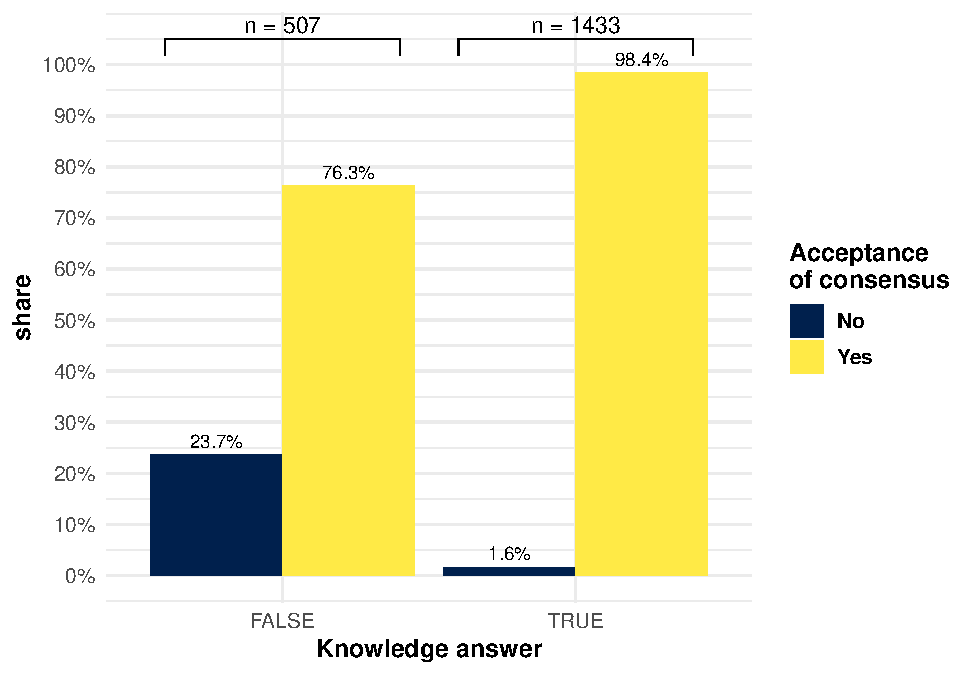
\includegraphics{output/figures/exp1-conditional-acceptance.pdf}
\caption{\label{fig:exp1-conditional-acceptance}Acceptance rates of scientific consensus, based on whether the initial response to the knowledge question was false or true.}
\end{figure}

For RQ3, we find a positive but small correlation between both science knowledge and trust in science (r = 0.29), and acceptance of scientific consensus and trust in science ( r = 0.27). The more people are knowledgeable about science and the more they tend to accept the scientific consensus, the more they tend to trust science. These correlations are relatively weak, which might be partly due to ceiling effects: As illustrated in Fig. \ref{fig:exp1-plot}, (i) most people do trust science, and (ii) that is true even among people with low knowledge or acceptance rates.

For RQ4, we find a negative correlation of similar magnitude between conspiracy thinking and science knowledge (r = -0.39), and conspiracy thinking and acceptance of scientific consensus ( r = -0.33).

In appendix XX we show that these results hold for our alternative measures of trust and conspiracy thinking. We also include more descriptive statistics, such as knowledge and acceptance by science questions.

Are trust in science and conspiracy thinking, respectively, associated with being more easily convinced of the scientific consensus? In our main analyses, we looked at correlations of acceptance across all observations. One possibility is that the associations between trust in science/conspiracy thinking and acceptance of scientific consensus are explained by science knowledge: People who give the right answer in the first place are more ready to accept the consensus, and trust in science/conspiracy thinking are mostly associated with this knowledge, but not with willingness to accept the consensus. To addressed this potential confound, in a non-preregistered analysis, we restricted our sample to cases where participants gave the wrong answer to the knowledge question. We than calculated the correlation between trust in science and average acceptance rate by participant. We find a slightly smaller negative correlation of acceptance with for conspiracy thinking (r = -0.14), and only a very small correlation for trust in science (r = 0.06). These associations are not statistically significant (see Appendix @ref:exp1).

The correlations of acceptance with

However, trust/CT is related to basic knowledge, so the fact that it is also related to the post feedback answer could just be a function of that.

\hypertarget{make-a-combined-plot-with-all-results}{%
\subsection{Make a combined plot with all results}\label{make-a-combined-plot-with-all-results}}



\begin{figure}
\centering
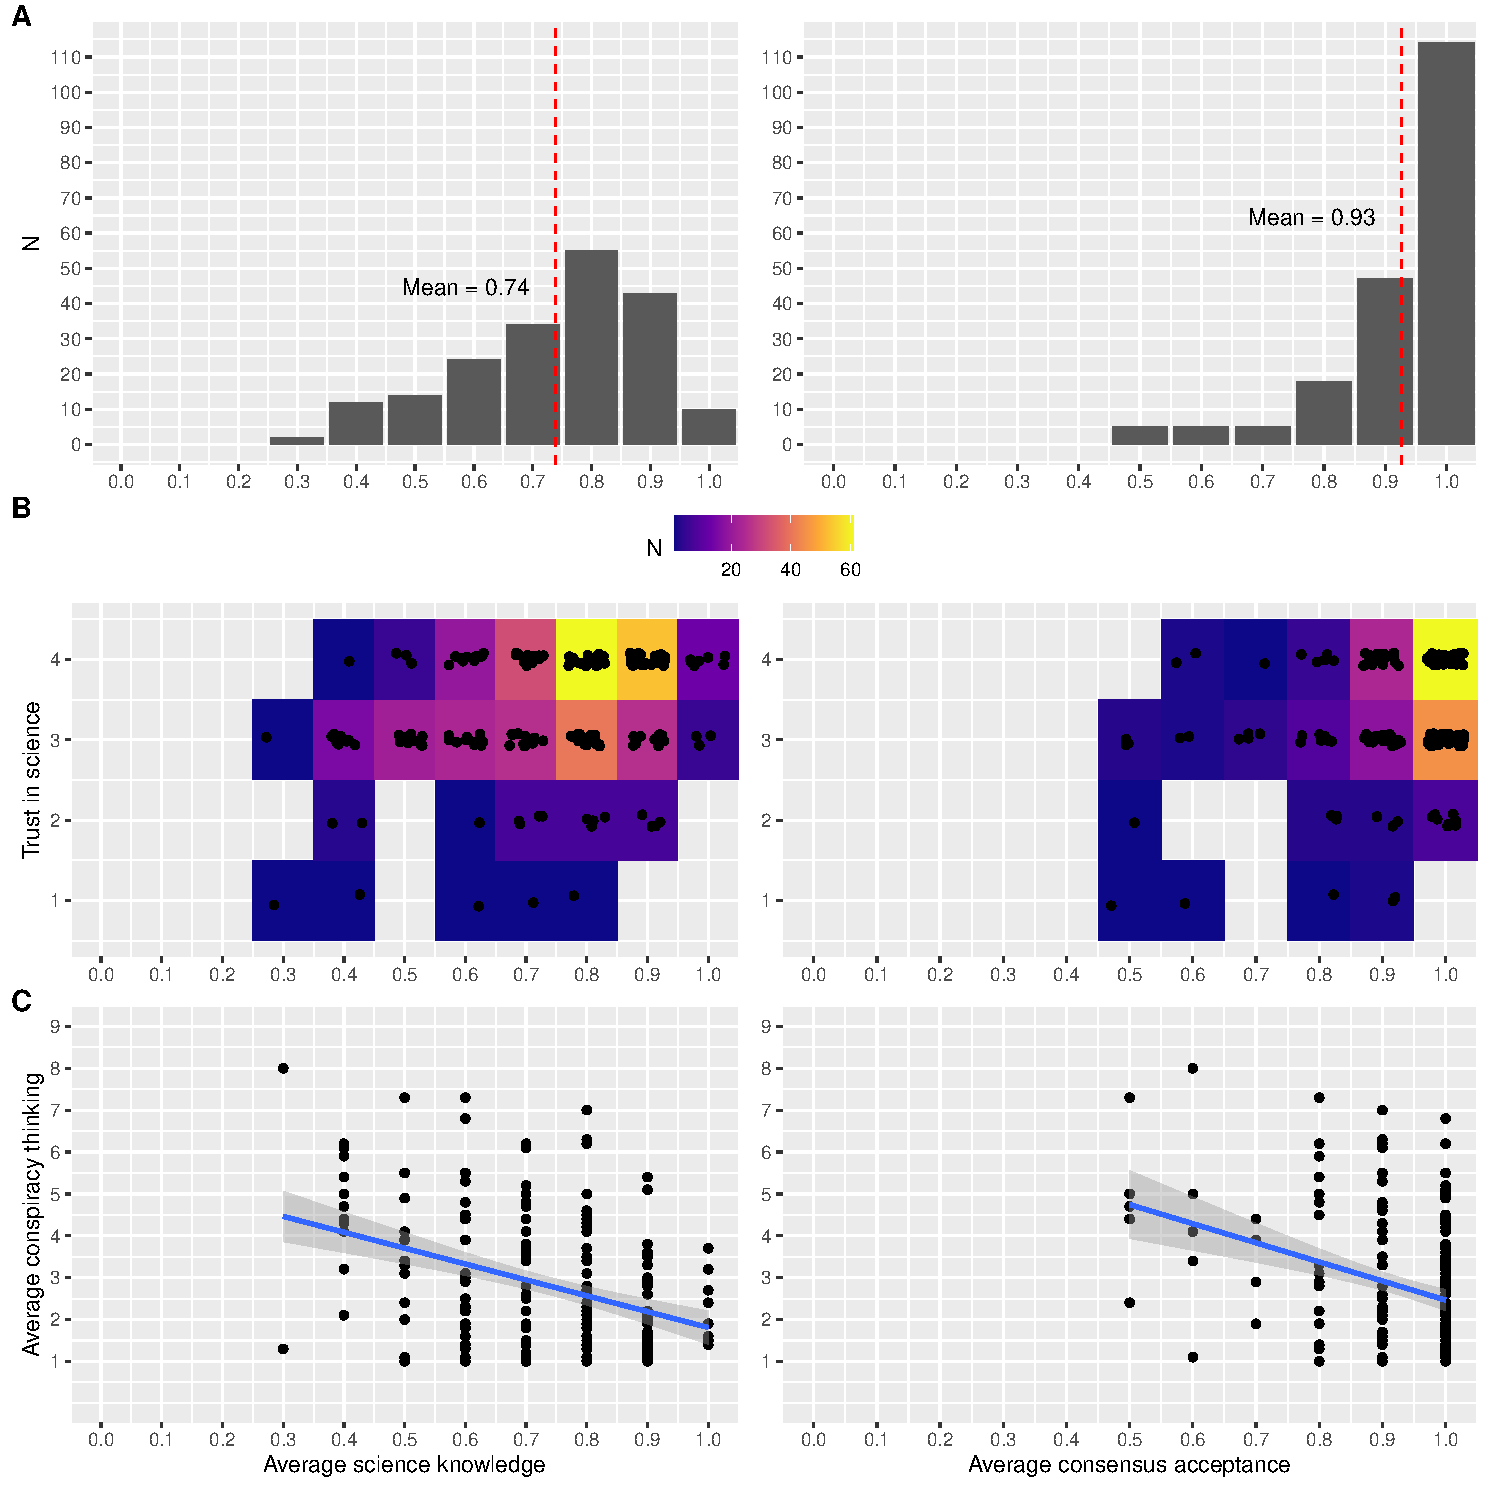
\includegraphics{output/figures/exp1-plot.pdf}
\caption{\label{fig:exp1-plot}\textbf{A} Shows the distribution of science knowledge (left) and acceptance of scientific consensus \textbf{B} Shows the relationship between trust in science and science knowledge/acceptance of scientific consensus \textbf{C} Shows the relationship between conspiracy thinking and science knowledge/acceptance of scientific consensus}
\end{figure}

\hypertarget{discussion}{%
\subsection{Discussion}\label{discussion}}

These results suggest that even when people do not know the answer to science questions, they tend to mostly accept the scientific consensus. Yet, in 23.7 \% of the cases, participants rejected the scientific consensus after having given the wrong answer, suggesting that simply stating the consensus is not sufficient to convince participants sometimes. In general, people with lower trust in science and who believe more in conspiracy theories tend to both know less about science and accept the scientific consensus less.

However, conditioning our analyses to initial false knowledge responses, i.e.~looking at change of opinion towards the scientific consensus, we find that trust in science is onl

(Experiment 1 Lou write up)

If we ask basic science questions, and we give feedback:
How many people accept the correct answer at the end?
Is that a function of TIS?
Is that a function of CT?

However, trust/CT is related to basic knowledge, so the fact that it is also related to the post feedback answer could just be a function of that.

So we look at who changes their minds. We still see an influence of CT (? do stats) (and of TIS?).

Takeaway:
Relatively high K in this population
After feedback even higher
But not at ceiling
Relation with TIS/CT, both in K, and in integrating feedback (?)

However, for those who don't accept the feedback, we don't know if it's because they don't trust us, or they don't trust science.
We can also try slightly more stringent attention checks (the fact that some people go from good to bad suggests some inattention)

\FloatBarrier

\hypertarget{references}{%
\section{References}\label{references}}

\hypertarget{refs}{}
\begin{CSLReferences}{1}{0}
\leavevmode\vadjust pre{\hypertarget{ref-bruderMeasuringIndividualDifferences2013}{}}%
Bruder, M., Haffke, P., Neave, N., Nouripanah, N., \& Imhoff, R. (2013). Measuring individual differences in generic beliefs in conspiracy theories across cultures: Conspiracy mentality questionnaire. \emph{Frontiers in Psychology}, \emph{4}. Retrieved from \url{https://www.frontiersin.org/articles/10.3389/fpsyg.2013.00225}

\leavevmode\vadjust pre{\hypertarget{ref-colognaTrustScientistsTheir2024}{}}%
Cologna, V., Mede, N. G., Berger, S., Besley, J., Brick, C., Joubert, M., \ldots{} Linden, D. S. van der. (2024). \emph{Trust in scientists and their role in society across 67 countries}. \url{https://doi.org/10.31219/osf.io/6ay7s}

\leavevmode\vadjust pre{\hypertarget{ref-lantianMeasuringBeliefConspiracy2016}{}}%
Lantian, A., Muller, D., Nurra, C., \& Douglas, K. M. (2016). Measuring Belief in Conspiracy Theories: Validation of a French and English Single-Item Scale. \emph{International Review of Social Psychology}, \emph{29}(1), 1. \url{https://doi.org/10.5334/irsp.8}

\leavevmode\vadjust pre{\hypertarget{ref-pennycookOverconfidentlyConspiratorialConspiracy2022}{}}%
Pennycook, G., Binnendyk, J., \& Rand, D. (2022). \emph{Overconfidently conspiratorial: Conspiracy believers are dispositionally overconfident and massively overestimate how much others agree with them}. \url{https://doi.org/10.31234/osf.io/d5fz2}

\end{CSLReferences}

\newpage

\hypertarget{appendix-appendix}{%
\appendix}


\hypertarget{exp1}{%
\section{Experiment 1}\label{exp1}}

\hypertarget{materials-1}{%
\subsection{Materials}\label{materials-1}}

\FloatBarrier

\hypertarget{conspiracy-scales-1}{%
\subsubsection{Conspiracy scales}\label{conspiracy-scales-1}}

Beside Belief in Conspiracy Theory Inventory (BCTI) by Pennycook et al. (2022) which report in the main study, we also assessed two other consipiracy thinking measures:

\begin{enumerate}
\def\labelenumi{\arabic{enumi}.}
\tightlist
\item
  The conspiracy mentality questionnaire (CMQ) by Bruder et al. (2013):
  I think that . . .
\end{enumerate}

\begin{itemize}
\tightlist
\item
  \ldots{} many very important things happen in the world, which the public is never informed about. - politicians usually do not tell us the true motives for their decisions.
\item
  \ldots{} government agencies closely monitor all citizens.
\item
  \ldots{} events which superficially seem to lack a connection are often the result of secret activities.
\item
  \ldots{} there are secret organizations that greatly influence political decisions.
\end{itemize}

{[}0\% - 100\%; 0 = certainly not, 100 = certain{]}

\begin{enumerate}
\def\labelenumi{\arabic{enumi}.}
\setcounter{enumi}{1}
\tightlist
\item
  The Single Item Conspiracy Beliefs Scale (SICBS) by Lantian et al. (2016) :
\end{enumerate}

\begin{itemize}
\tightlist
\item
  I think that the official version of the events given by the authorities very often hides the truth. {[}1-9; 1 = Completely false, 5 = Unsure, 9 = Completely true{]}
\end{itemize}

\hypertarget{trust-in-science-1}{%
\subsubsection{Trust in science}\label{trust-in-science-1}}

We rely on three items

\begin{enumerate}
\def\labelenumi{\arabic{enumi}.}
\item
  How much do you trust scientists in this country? Do you trust them a lot, some, not much, or not at all? {[}1 = Not at all, 2 = Not much, 3 = Some, 4 = A lot{]}
\item
  In general, would you say that you trust science a lot, some, not much, or not at all? {[}1 = Not at all, 2 = Not much, 3 = Some, 4 = A lot{]}
\item
  How much confidence do you have in scientists to act in the best interests of the public? {[}1-5; 1 = No confidence at all, 5 = A great deal of confidence{]}
\end{enumerate}

\hypertarget{comparing-items}{%
\subsection{Comparing items}\label{comparing-items}}

Make correlation table

\hypertarget{conspiracy-theories}{%
\subsubsection{Conspiracy theories}\label{conspiracy-theories}}

Table \ref{tab:correlation-conspiracy} shows the correlations of the three different scales assessing conspiracy thinking.

\begin{table}[h]

\begin{center}
\begin{threeparttable}

\caption{\label{tab:correlation-conspiracy}Correlations of the three different scales assessing conspiracy thinking}

\begin{tabular}{llll}
\toprule
 & \multicolumn{1}{c}{BCTI} & \multicolumn{1}{c}{CMQ} & \multicolumn{1}{c}{SICBS}\\
\midrule
BCTI & 1.00 & 0.58 & 0.56\\
CMQ & 0.58 & 1.00 & 0.77\\
SICBS & 0.56 & 0.77 & 1.00\\
\bottomrule
\end{tabular}

\end{threeparttable}
\end{center}

\end{table}

\hypertarget{trust-in-science-2}{%
\subsubsection{Trust in science}\label{trust-in-science-2}}

Table \ref{tab:correlation-trust} shows the correlations of the three different items measuring trust in science.

\begin{table}[h]

\begin{center}
\begin{threeparttable}

\caption{\label{tab:correlation-trust}Correlations of the three different items measuring trust in science}

\begin{tabular}{llll}
\toprule
 & \multicolumn{1}{c}{wgm\_sciencegeneral} & \multicolumn{1}{c}{wgm\_scientists} & \multicolumn{1}{c}{pew}\\
\midrule
wgm\_sciencegeneral & 1.00 & 0.85 & 0.75\\
wgm\_scientists & 0.85 & 1.00 & 0.82\\
pew & 0.75 & 0.82 & 1.00\\
\bottomrule
\end{tabular}

\end{threeparttable}
\end{center}

\end{table}

\hypertarget{correlations-with-alternative-measures}{%
\subsection{Correlations with alternative measures}\label{correlations-with-alternative-measures}}

Table \ref{tab:correlations-outcomes} shows the correlations between knowledge and acceptance, respectively, and outcome variables.

\begin{table}[tbp]

\begin{center}
\begin{threeparttable}

\caption{\label{tab:correlations-outcomes}Correlations between knowledge and acceptance, respectively, and outcome variables}

\begin{tabular}{lll}
\toprule
outcome & \multicolumn{1}{c}{Correlation with knowledge} & \multicolumn{1}{c}{Correlation with acceptance}\\
\midrule
BCTI 
(main conspiracy measure) & -0.39 & -0.33\\
CMQ & -0.11 & -0.07\\
SICBS & -0.10 & -0.09\\
WGM trust scientists & 0.23 & 0.26\\
WGM trust general 
(main trust measure) & 0.29 & 0.27\\
PEW trust scientists & 0.16 & 0.21\\
\bottomrule
\end{tabular}

\end{threeparttable}
\end{center}

\end{table}

\hypertarget{results-conditional-on-false-responses}{%
\subsection{Results conditional on false responses}\label{results-conditional-on-false-responses}}

Table \ref{tab:false-response-regression} shows the correlations between acceptance and outcome variables based on linear regression models on standardized values.

\begin{table}

\caption{\label{tab:false-response-regression}Based on false response data only, correlations between acceptance and outcome variables based on linear regression models on standardized values}
\centering
\begin{tabular}[t]{lcccccc}
\toprule
  & BCTI\_avg & CMQ\_avg & SICBS & wgm\_scientists & wgm\_sciencegeneral & pew\\
\midrule
(Intercept) & 0.000 & 0.000 & 0.000 & 0.000 & 0.000 & 0.000\\
 & (0.073) & (0.074) & (0.074) & (0.073) & (0.074) & (0.074)\\
avg\_acceptance & -0.139+ & 0.008 & -0.028 & 0.108 & 0.064 & 0.056\\
 & (0.073) & (0.074) & (0.074) & (0.074) & (0.074) & (0.074)\\
\midrule
Num.Obs. & 184 & 184 & 184 & 184 & 184 & 184\\
R2 & 0.019 & 0.000 & 0.001 & 0.012 & 0.004 & 0.003\\
R2 Adj. & 0.014 & -0.005 & -0.005 & 0.006 & -0.001 & -0.002\\
AIC & 523.6 & 527.2 & 527.0 & 525.0 & 526.4 & 526.6\\
BIC & 533.2 & 536.8 & 536.7 & 534.7 & 536.1 & 536.2\\
Log.Lik. & -258.801 & -260.578 & -260.512 & -259.506 & -260.204 & -260.295\\
RMSE & 0.99 & 1.00 & 1.00 & 0.99 & 1.00 & 1.00\\
\bottomrule
\multicolumn{7}{l}{\rule{0pt}{1em}+ p $<$ 0.1, * p $<$ 0.05, ** p $<$ 0.01, *** p $<$ 0.001}\\
\end{tabular}
\end{table}


\end{document}
